% Reference draft (v2) of a research paper for the Yale STEM Research Supplement.
% All results come from ../model, ../competition and ../mine_example.
% Compile with: latexmk -xelatex Escaping_a_Flooding_Mine_v2.tex
% Orange [TO DO] / [CONFIRM] markers are items only the student can supply.
\documentclass[11pt,a4paper]{article}

\usepackage[top=2.4cm,bottom=2.4cm,left=2.5cm,right=2.5cm,headheight=14pt]{geometry}
\usepackage{amsmath,amssymb,amsthm}
\usepackage{fontspec}
\usepackage{unicode-math}
\setmainfont{Times New Roman}
\setmathfont{STIX Two Math}
\setsansfont{Arial}

\usepackage{graphicx}
\usepackage{booktabs,array,tabularx}
\usepackage{tikz}
\usetikzlibrary{arrows.meta,positioning}
\usepackage{caption}
\captionsetup{font=small, labelfont=bf}
\usepackage{xcolor}
\usepackage{enumitem}
\usepackage[most]{tcolorbox}
\usepackage{fancyhdr}
\usepackage[hidelinks]{hyperref}

\linespread{1.12}
\setlength{\parskip}{0.35em}
\hyphenation{Dijkstra}

\newcommand{\todo}[1]{\leavevmode{\color{orange!85!black}\sffamily\small[TO DO: #1]}}
\newcommand{\confirm}[1]{\leavevmode{\color{orange!85!black}\sffamily\small[CONFIRM: #1]}}

\newtheorem{proposition}{Proposition}
\newtheorem{lemma}{Lemma}
\newtheorem{theorem}{Theorem}
\newtheorem{corollary}{Corollary}
\theoremstyle{remark}
\newtheorem*{remark}{Remark}

\pagestyle{fancy}
\fancyhf{}
\fancyhead[L]{\color{gray}\sffamily\scriptsize Reference draft for tutor review --- to be rewritten by the student before submission}
\fancyhead[R]{\color{gray}\sffamily\scriptsize \thepage}
\renewcommand{\headrulewidth}{0pt}

\newcommand{\tin}{t_{\mathrm{in}}}
\newcommand{\tblock}{t_{\mathrm{block}}}
\newcommand{\tfull}{t_{\mathrm{full}}}

\begin{document}

\begin{center}
  {\LARGE\bfseries Escaping a Flooding Mine:\\[3pt]
  \Large A Volume-Conserving Flood Model and\\[1pt] Time-Dependent Shortest Paths}\\[10pt]
  {\large [Student Name]}\\[2pt]
  {\small [School], [City, Country]\quad$\cdot$\quad [Month Year]}
\end{center}

\begin{tcolorbox}[colback=gray!6, colframe=gray!50, boxrule=0.5pt, arc=2pt, left=6pt, right=6pt, top=4pt, bottom=4pt, fontupper=\small]
\textbf{Origin of this paper.} This paper grows out of a team paper written in Chinese for Problem~D of the 2025 China Undergraduate Mathematical Contest in Modeling (CUMCM), a 72-hour competition. The team was [Student Name], [Teammate A] and [Teammate B] \confirm{advisor, if any; award, if any}. During the competition we built a graph model of the tunnels, an event-driven flood simulation and an escape-routing program; my own part was \todo{state precisely}. After the competition I found that our flood simulation did not conserve water, replaced it with a volume-conserving model (Section~\ref{sec:flood}), proved the properties in Sections~\ref{sec:props} and~\ref{sec:fifo}, replaced the approximate walking-time calculation with an exact one, reran Problems~1--4 on the original data, and applied the method to a real mine plan (Section~\ref{sec:example}). All results in this paper come from the new code. Appendix~A lists every change from the competition version. \todo{say honestly which of these steps you did yourself, how the paper was translated, and which tools (including AI) you used}
\end{tcolorbox}

\begin{abstract}
\noindent When water bursts into a mine, the tunnels that miners need to escape are the ones that are filling up. I model a mine as a graph of tunnels and simulate the flood with an event-driven algorithm in which water spreads into level and downhill tunnels, splits equally at junctions, and backs up from dead ends. Unlike the algorithm my team wrote during a 72-hour competition, this model conserves water: the stored volume always equals the inflow, so the network fills exactly at (total volume)/(inflow) --- 35 days for the competition networks, where the competition algorithm predicted that some junctions would stay dry for thousands of years. The flood determines when each tunnel becomes wet and when it becomes impassable, so the time needed to walk through a tunnel depends on when a miner enters it. I prove that a miner who enters a tunnel later never leaves it earlier. This first-in, first-out property makes Dijkstra's algorithm exact on the time-dependent network, shows that waiting never helps, and makes ``the latest safe moment to start'' well defined. On the competition networks all six miners escape within 12--20 minutes of the inrush, five of them on routes that stay completely dry; after a second inrush, re-planning saves up to 7.6 minutes compared with keeping the old route. On an anonymized real mine plan, with 248\,km of tunnels extracted automatically from a CAD drawing, flood-aware routes are up to 40\% faster than the shortest route in a dry mine, and the miner nearest the inrush has a way out only if alerted within 4 minutes 40 seconds.
\end{abstract}

% =====================================================================
\section{Introduction}

Water inrush is one of the major hazards of underground coal mining: it is sudden, hard to predict, and the water quickly blocks the tunnels that lead out of the mine \cite{guo}. Two questions follow. How does the water spread through the tunnel network? And, given that spread, which route gets each miner out fastest? The questions are coupled: the best route depends on when each tunnel becomes impassable, and that depends on the flood.

Problem~D of CUMCM 2025 \cite{cumcm} posed these questions for two networks of 663 junctions and 977 tunnels each. Tunnels are 4\,m wide and 3\,m high; water bursts in at $Q = 30\ \mathrm{m^3/min}$, advances at a depth of 0.1\,m and at a junction ``splits equally among the level and downhill tunnels''. Miners walk at 4\,m/s in dry tunnels; in water up to 0.3\,m deep they walk at 2\,m/s with the flow and 1\,m/s against it; deeper water is impassable. They start one minute after the inrush. Problems~1--2 ask for the flood and the escape routes; Problems~3--4 add a second inrush a few minutes later and ask for re-planned routes.

\paragraph{Contributions.}
\begin{enumerate}[leftmargin=2em, itemsep=1pt, topsep=2pt]
  \item A \textbf{volume-conserving} event-driven flood model that follows the problem's rules and fills dead ends first (Section~\ref{sec:flood}). I show why the competition algorithm violated conservation and what that did to its predictions.
  \item Three properties of the flood model: exact scaling with the inflow, the geometric slowdown of the spreading front, and an exact formula for when the network is full (Propositions~1--3).
  \item An \textbf{exact} time-dependent routing model and a proof that it is first-in, first-out, so that Dijkstra's algorithm is exact, waiting never helps, and the latest safe start time is well defined (Lemma~1, Theorem~1, Corollary~1).
  \item Complete solutions of Problems~1--4, a sensitivity analysis and numerical checks of every proposition.
  \item A worked example on an anonymized real mine plan, from a CAD drawing to escape routes (Section~\ref{sec:example}).
\end{enumerate}

\begin{figure}[htbp]
  \centering
  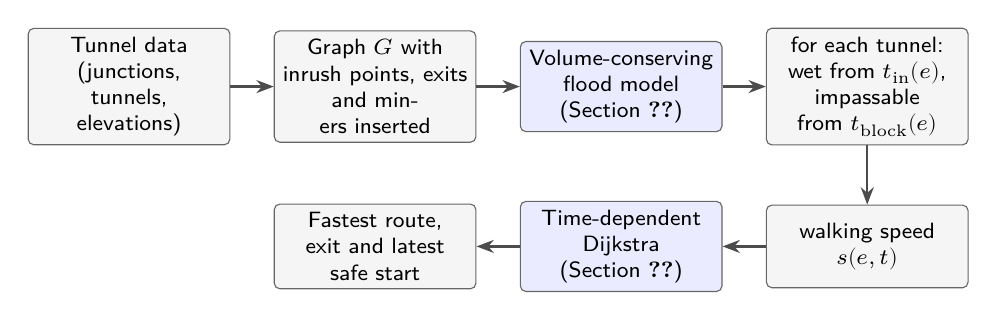
\begin{tikzpicture}[
      font=\sffamily\footnotesize,
      box/.style={draw=black!60, rounded corners=2pt, fill=#1, align=center, minimum height=1.05cm, text width=2.35cm, inner sep=3pt},
      box/.default=gray!8,
      arr/.style={-{Stealth[length=2.2mm]}, thick, black!70},
      node distance=0.55cm,
    ]
    \node[box] (data) {Tunnel data\\(junctions, tunnels,\\elevations)};
    \node[box, right=of data] (graph) {Graph $G$ with\\inrush points, exits\\and miners inserted};
    \node[box=blue!8, right=of graph] (flood) {Volume-conserving\\flood model\\(Section~\ref{sec:flood})};
    \node[box, right=of flood] (times) {for each tunnel:\\wet from $\tin(e)$,\\impassable from $\tblock(e)$};
    \node[box, below=0.75cm of times] (speed) {walking speed\\$s(e,t)$};
    \node[box=blue!8, left=of speed] (route) {Time-dependent\\Dijkstra\\(Section~\ref{sec:routing})};
    \node[box, left=of route] (out) {Fastest route,\\exit and latest\\safe start};
    \draw[arr] (data) -- (graph);
    \draw[arr] (graph) -- (flood);
    \draw[arr] (flood) -- (times);
    \draw[arr] (times) -- (speed);
    \draw[arr] (speed) -- (route);
    \draw[arr] (route) -- (out);
  \end{tikzpicture}
  \caption{How the two models connect. The flood is simulated once; its output turns the tunnel network into a network whose travel times change with time.}
  \label{fig:pipeline}
\end{figure}

% =====================================================================
\section{The Tunnel Networks}

Each network is a list of junctions with coordinates $(x,y,z)$ and a list of tunnels joining pairs of junctions. I store it as an undirected graph $G=(P,H)$ and give each tunnel $e$ its 3D length $L_e$. Both networks have the same layout --- 663 junctions, 977 tunnels, 125.6\,km of tunnel --- and three quarters of the junctions (501 of 663) have degree~3. In Network~1 every junction is at the same elevation; Network~2 is three-dimensional, with elevations from 0 to 71.5\,m (Figure~\ref{fig:3d}).

\begin{figure}[htbp]
  \centering
  \begin{minipage}{0.48\textwidth}\centering
    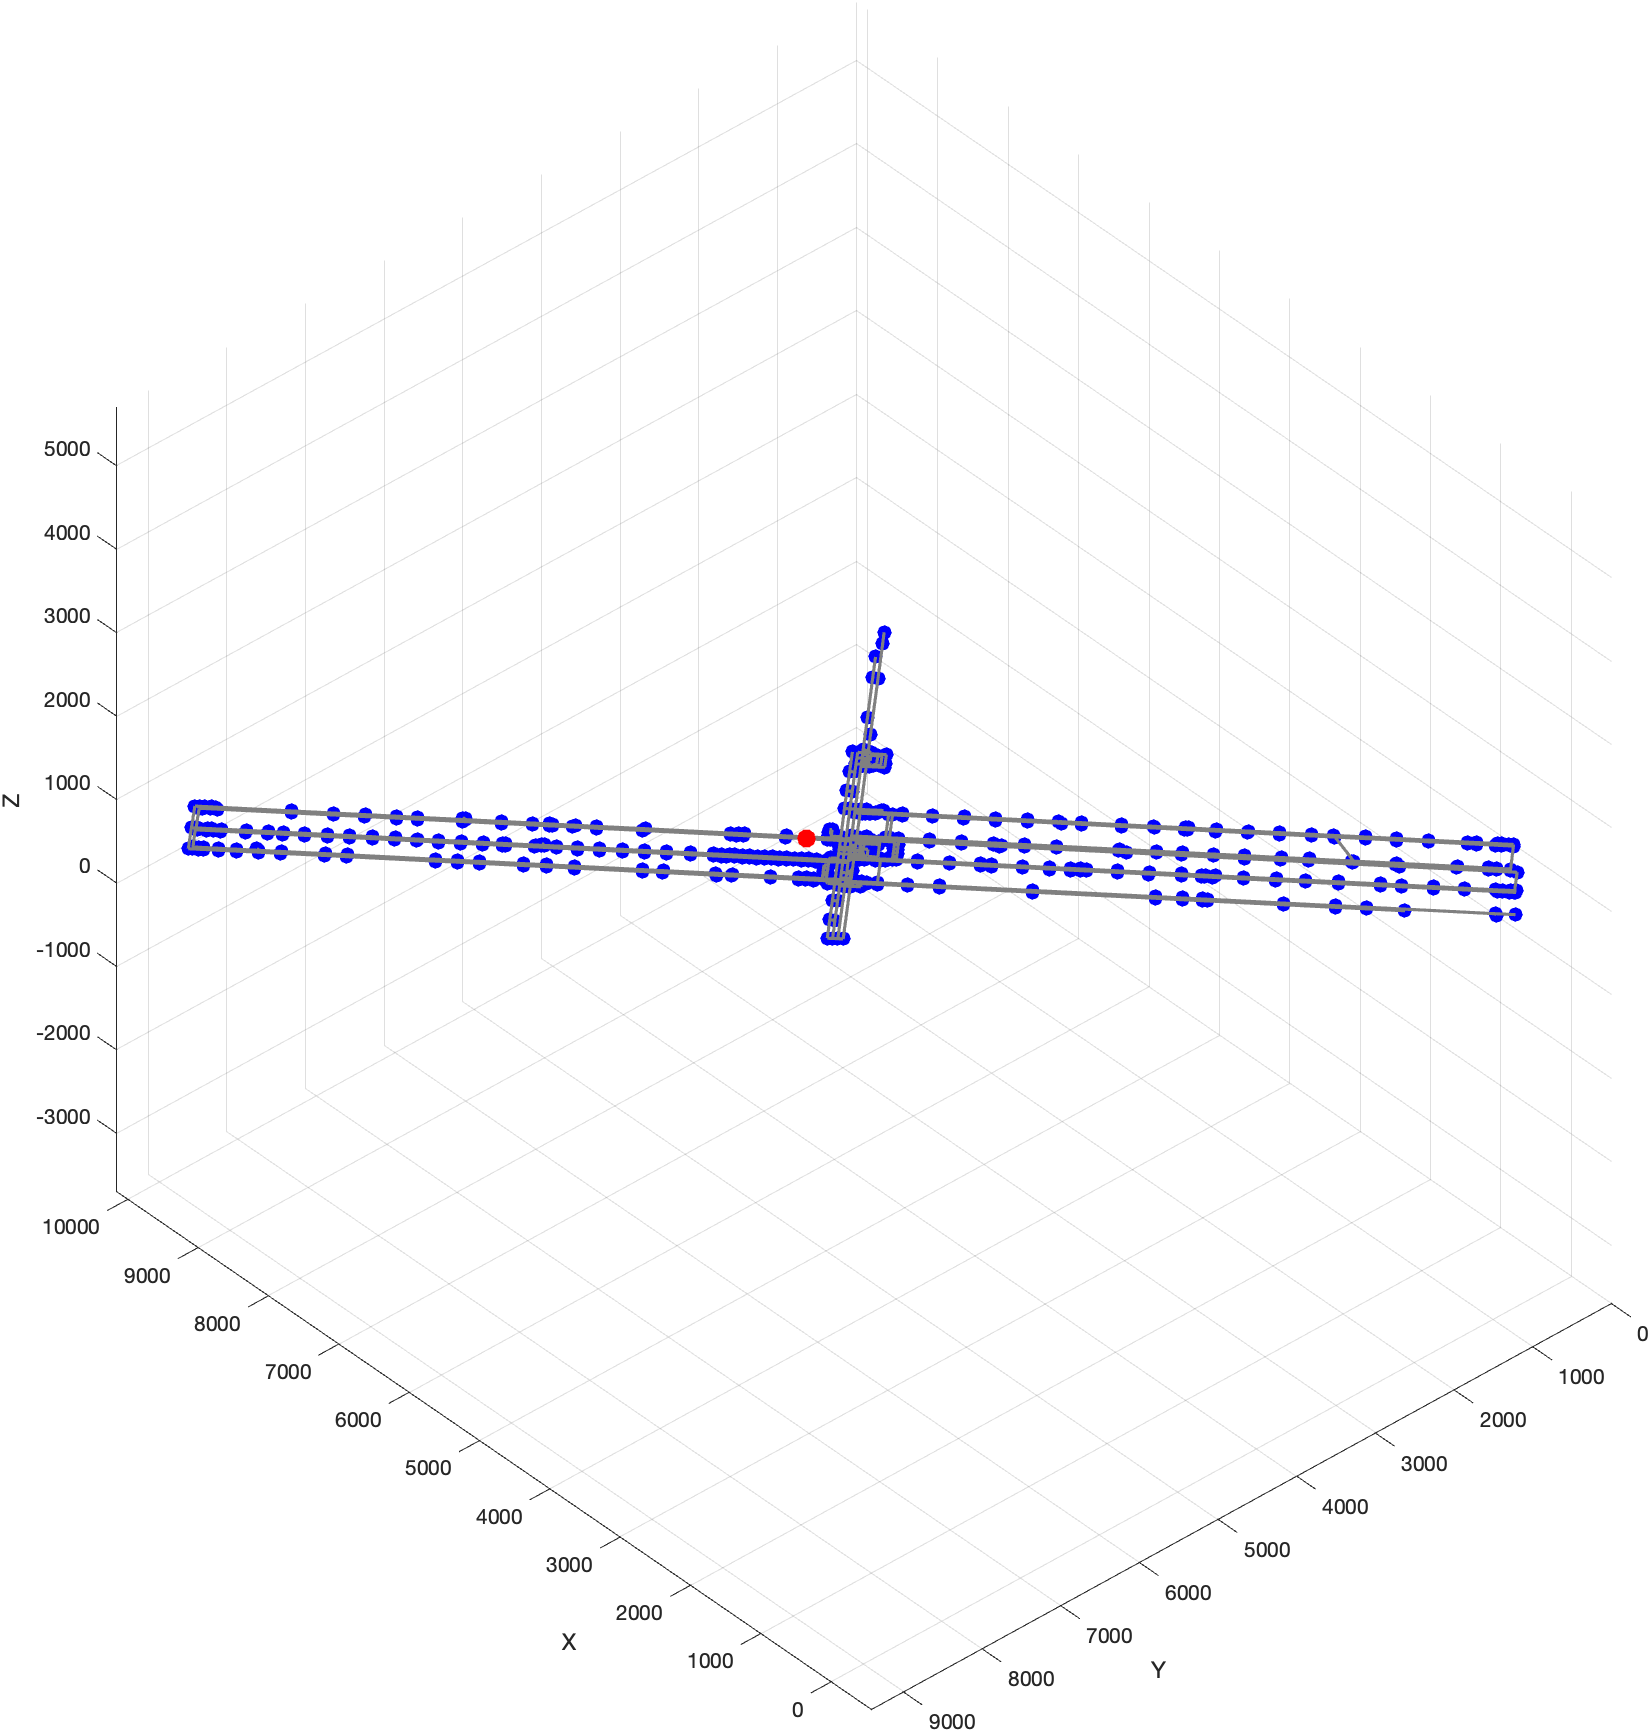
\includegraphics[width=\linewidth]{figures/fig03_att1_3d.png}
  \end{minipage}\hfill
  \begin{minipage}{0.48\textwidth}\centering
    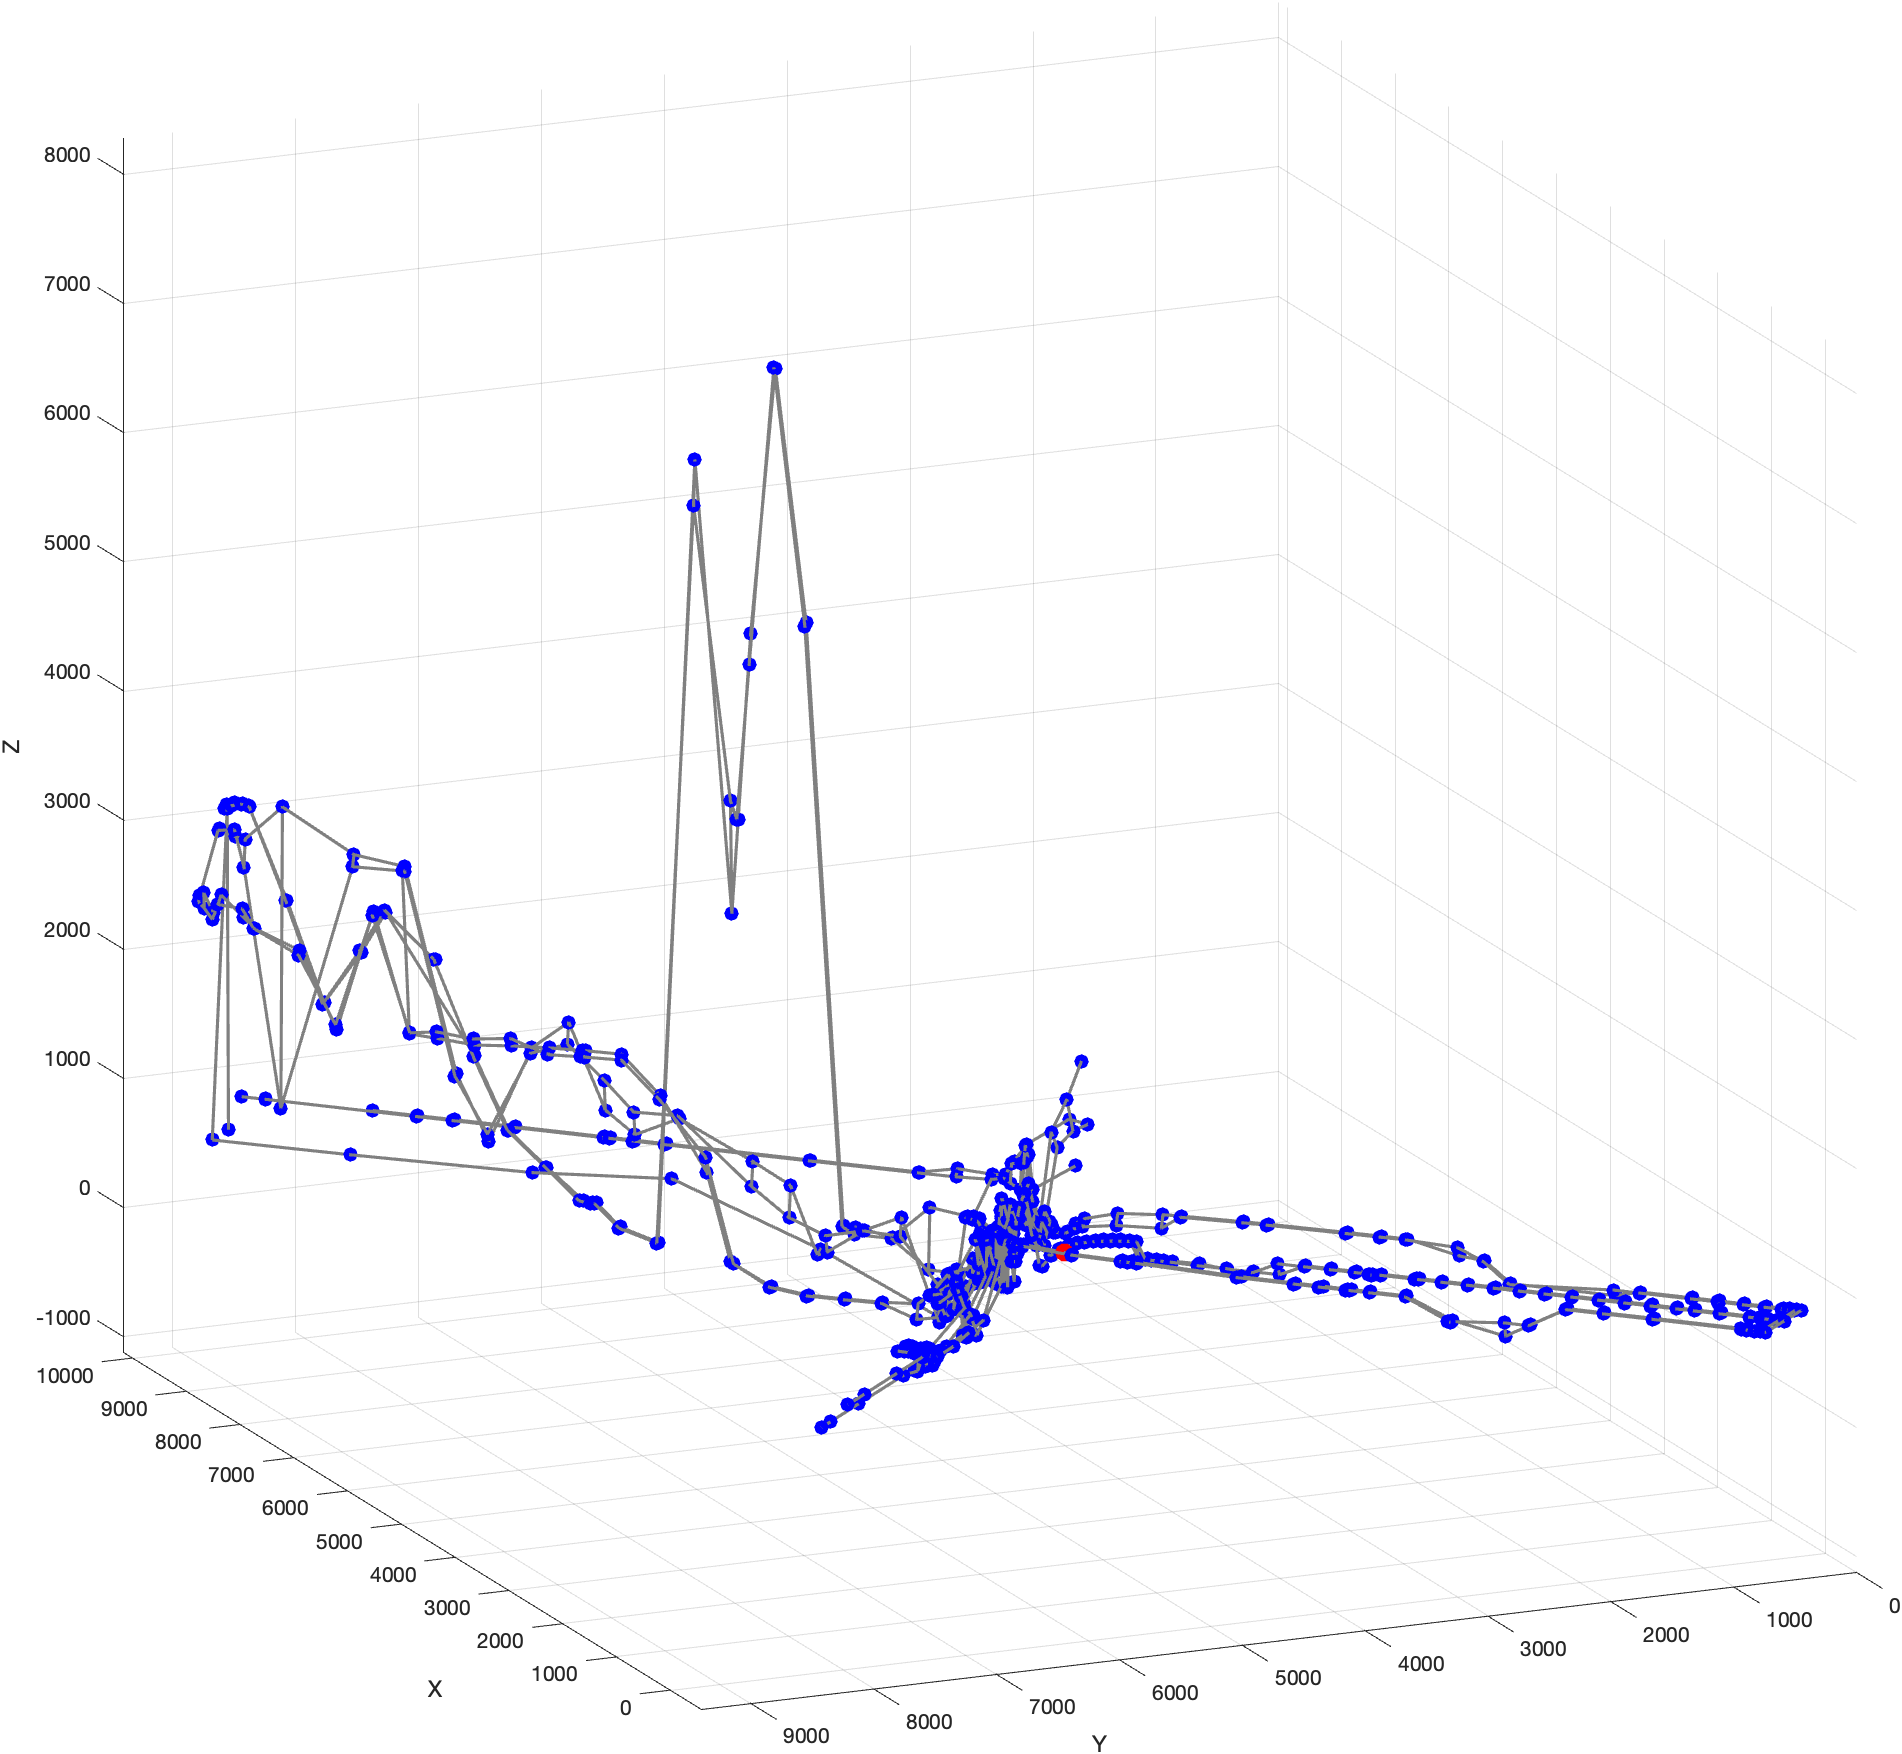
\includegraphics[width=\linewidth]{figures/fig04_att2_3d.png}
  \end{minipage}
  \caption{Network~1 (left, flat) and Network~2 (right, three-dimensional); the red dot is the inrush point. Elevation is exaggerated 100 times.}
  \label{fig:3d}
\end{figure}

\paragraph{Inserting points into tunnels.} Inrush points, exits and miners are given by coordinates, usually inside a tunnel. I project each point onto the nearest tunnel and split that tunnel there, adding the point as a junction of degree~2 (if it falls on an existing junction, I use that junction). All given points lie on the network to within 0.016\,m, consistent with coordinates rounded to two decimals. After this step the inrush point is an ordinary node, and the simulation needs no special case for it.

% =====================================================================
\section{Flood Model}\label{sec:flood}

\subsection{What went wrong in the competition version}
The competition algorithm processed ``the water front reaches the end of tunnel $e$'' events with a priority queue. At such an event it did two things with the flow $q$ that had arrived through $e$: it passed $q$ on, split among the next tunnels, \emph{and} it started filling $e$ at rate $q$. Already for two tunnels in series, while the second one is being covered the network stores water at rate $2q$ although only $q$ flows in. On large networks the flow at the tips of the front becomes tiny while the rest of the water is counted twice, and the predicted times become absurd: on Network~1 the competition algorithm gives a median arrival time of 445 days and a last junction reached after about 16{,}000 years; on Network~2 its rule ``water never enters an uphill tunnel'' leaves 635 of the 663 junctions dry forever.

\subsection{Rules of the new model}
Let $W=4$\,m and $H=3$\,m be the tunnel width and height and $h_0=0.1$\,m the depth of the advancing front. At every moment each tunnel is \emph{dry}, \emph{being covered} (a front at depth $h_0$ is advancing), \emph{passing water on} (covered, delivering its inflow to its far end), \emph{storing} (its water level rises) or \emph{full}. Each wet junction remembers the tunnel that first brought it water.
\begin{enumerate}[leftmargin=2em, itemsep=2pt, topsep=2pt, label=\textbf{R\arabic*.}]
  \item \textbf{Spreading.} A wet junction splits all the water reaching it equally among its \emph{outlets}: the tunnels at it that are not full and are level or downhill (problem statement), apart from the one feeding it. Only if there are none do uphill tunnels count; water enters an uphill tunnel from below and fills it.
  \item \textbf{Passing on or storing.} When a tunnel is covered, it passes its water on if its far end was still dry (the far end becomes wet); if the far end was already wet --- a loop, or two fronts meeting --- it stores the water.
  \item \textbf{Backing up.} If a junction receives water but has no outlet, the tunnel feeding it stops passing water on and stores it. A full tunnel takes no more water, so water backs up from dead ends toward the source. If every tunnel at an inrush point is full, its inflow runs through the flooded tunnels to the nearest junction where there is still room.
  \item \textbf{Rising over a hill.} An uphill tunnel that has filled delivers its water to its upper end if that end is dry.
\end{enumerate}
The stored volume of a tunnel only grows, and its depth is the stored volume divided by $W L_e$. For each tunnel the model records the time water first enters it, $\tin(e)$, and the time its depth first exceeds 0.3\,m, $\tblock(e)$; these are all the routing model needs.

\subsection{Event-driven simulation}
Between events every flow rate is constant, so each tunnel's volume grows linearly. The simulation jumps from event to event:

\begin{tcolorbox}[colback=gray!4, colframe=gray!45, boxrule=0.4pt, arc=1pt, fontupper=\small, title={\small Algorithm 1: volume-conserving flood simulation}, coltitle=black, colbacktitle=gray!15, left=5pt]
\begin{enumerate}[label=\arabic*., leftmargin=1.6em, itemsep=0pt, topsep=0pt]
  \item \emph{Distribute.} Visit the wet junctions in the order they became wet (so every feeding tunnel is handled before the junction it feeds). Split each junction's inflow --- from an inrush point and from its feeding tunnel --- among its outlets (R1); apply R3 where a junction has no outlet.
  \item \emph{Next event.} For every tunnel receiving water, compute when its volume reaches the next threshold: $W h_0 L_e$ (covered), $0.3\,W L_e$ (impassable) or $H W L_e$ (full). Take the earliest of these and of the start of the next inrush.
  \item \emph{Advance} all volumes to that time; record $\tblock$ or $\tfull$; apply R2 and R4 to tunnels that became covered or full.
  \item Repeat until the network is full.
\end{enumerate}
\end{tcolorbox}

Each tunnel passes each threshold once, so there are $O(|H|)$ events, and each costs $O(|P|+|H|)$. A complete flood of a competition network takes about one second.

\subsection{Three properties}\label{sec:props}

\begin{proposition}[Scaling with the inflow]
For a single inrush point starting at $t=0$, multiplying the inflow $Q$ by $\lambda>0$ multiplies every time computed by Algorithm~1 by exactly $1/\lambda$.
\end{proposition}
\begin{proof}
Every flow rate is $Q$ times a fraction that depends only on the graph and on the modes of the tunnels, and every event time is the current time plus (threshold volume $-$ current volume)/(rate). If the two runs have gone through the same events with all times multiplied by $1/\lambda$, all volumes agree and all rates differ by the factor $\lambda$, so the next event is the same and happens at $1/\lambda$ times the time. By induction, the runs coincide up to this time scaling.
\end{proof}

So 10\% more inflow makes every flood time exactly $1-1/1.1 \approx 9.1\%$ shorter, and a ten times larger inrush is the same flood played ten times faster. The scaling fails with a second inrush at a fixed delay.

\begin{proposition}[Slowdown of the spreading front]
Follow the front along tunnels $e_1,\dots,e_k$ leaving an inrush point of degree~2, before any tunnel stores water, and let $m_i$ be the number of outlets at the far end of $e_i$. Then $e_k$ receives $q_k = Q/(2\,m_1\cdots m_{k-1})$ and is covered after $W h_0 L_{e_k}/q_k$.
\end{proposition}
\begin{proof}
Each tunnel at the inrush point receives $Q/2$, and each junction divides its inflow by $m_i$ (R1).
\end{proof}

At degree-3 junctions $m_i=2$, so the flow halves at every junction and the front slows down geometrically: far from the source it creeps. In the competition algorithm this was the whole story, which is why its times grew without bound. Conservation changes that:

\begin{proposition}[Conservation and the filling time]
Let inrushes start at times $s_j$ with inflows $Q_j$, in a connected network whose tunnels hold a total volume $V = \sum_e W H L_e$. As long as some tunnel is not full, the water stored in the network at time $t$ is exactly $\sum_j Q_j (t-s_j)^+$. Hence the last tunnel fills at the time $t^*$ with $\sum_j Q_j (t^*-s_j) = V$; for one inrush, $t^* = V/Q$.
\end{proposition}
\begin{proof}
At every moment, rules R1--R4 send each junction's inflow either into tunnels that store it or onward to other junctions; flow is never created or destroyed. It can only fail to find a place if a junction has inflow, no outlet, and no feeding tunnel to back up into. That junction's tunnels are all full; by R3 its water moves through full tunnels to the nearest junction with room, which exists while some tunnel is not full, because the network is connected. So the storage rate always equals the total inflow.
\end{proof}

For the competition networks ($V = 4\times 3 \times 125.6\,\mathrm{km} = 1.51\times10^6\ \mathrm{m^3}$, $Q = 0.5\ \mathrm{m^3/s}$) this gives $t^* = 837$ hours, about 35 days, and the simulation's last tunnel fills at this time to 12 significant digits.

% =====================================================================
\section{Escape-Routing Model}\label{sec:routing}

\subsection{Walking through a tunnel}
A miner walks at 4\,m/s in a tunnel that is still dry ($t < \tin(e)$), at $u_e = 2$\,m/s (with the flow) or 1\,m/s (against it) once water has entered ($\tin(e) \le t \le \tblock(e)$), and cannot walk on after the depth exceeds 0.3\,m. The direction of the flow in each tunnel comes from the flood model. Treating the whole tunnel as wet from the moment water enters it is the cautious choice. Since the speed changes at most once, the exit time when entering at time $t$ has a closed form:
\begin{equation}
  a_e(t) = \begin{cases}
    t + L_e/4, & L_e \le 4\,(\tin - t)^+,\\[2pt]
    \max(t,\tin) + \dfrac{L_e - 4(\tin - t)^+}{u_e}, & \text{otherwise},
  \end{cases}
  \label{eq:exit}
\end{equation}
and $a_e(t) = \infty$ if this exceeds $\tblock(e)$. The competition code instead divided each tunnel into 20 segments and used the speed at the start of each segment. That can reverse a feasibility decision: for a 20\,m tunnel that becomes wet at 4.1\,s ($u_e = 2$\,m/s), the exact exit time is 5.9\,s but the segment method gives 5.75\,s, so a tunnel that becomes impassable at 5.77\,s would wrongly be judged passable.

\subsection{Why Dijkstra's algorithm is exact here}\label{sec:fifo}

\begin{lemma}[First in, first out]
For every tunnel and direction, $a_e$ is non-decreasing: if $t_1 \le t_2$ then $a_e(t_1) \le a_e(t_2)$.
\end{lemma}
\begin{proof}
The walking speed in a tunnel depends only on time, not on the position in the tunnel, and it never increases (water only rises). Let two miners enter at $t_1 \le t_2$. At time $t_2$ the first is ahead (or already out); from then on both always walk at the same speed, so the gap never closes and the first leaves no later. If the tunnel becomes impassable before the first miner is out, it does so before the second is out too, and both exit times are $\infty$.
\end{proof}

\begin{theorem}
Run Dijkstra's algorithm from the miner's position with label $\tau(\text{start}) = t_0$, where settling a junction $u$ updates each neighbour by $\tau(v) \gets \min\{\tau(v), a_{uv}(\tau(u))\}$. Every settled label is the earliest possible arrival time at that junction, and waiting at a junction never gives an earlier arrival.
\end{theorem}
\begin{proof}
\emph{Waiting:} leaving $u$ at $t' \ge t$ gives $a_{uv}(t') \ge a_{uv}(t)$ by Lemma~1.
\emph{Correctness:} suppose all settled junctions have correct labels, $u$ is the next to be settled, and some route reaches $u$ at $T < \tau(u)$. Let $(x,y)$ be the first tunnel on that route leaving the settled set. The route reaches $x$ no earlier than $\tau(x)$, so by Lemma~1 it reaches $y$ no earlier than $a_{xy}(\tau(x))$, which has already been used to update $\tau(y)$. Since $a_e(t) \ge t$, times along the route never decrease, so $\tau(y) \le T < \tau(u)$ and the algorithm would settle $y$ before $u$ --- a contradiction.
\end{proof}

The search stops at the first exit it settles, which is the exit the miner can reach soonest. Such time-dependent shortest paths, and the role of the first-in, first-out property, are known from transportation research \cite{dreyfus, kaufman, orda}; the point here is that the property follows directly from the flood model.

\begin{corollary}[Latest safe start]
For a fixed route, the start times from which it reaches the exit form an interval $(-\infty, D]$; the same holds for ``some route reaches an exit''.
\end{corollary}
\begin{proof}
The exit time along a route is a composition of non-decreasing functions $a_e$, so it is non-decreasing in the start time; if a start at $t$ succeeds, so does any earlier start.
\end{proof}

For a fixed route, $D$ is computed exactly by inverting~\eqref{eq:exit} tunnel by tunnel from the exit backwards. For ``some route'', the corollary justifies bisection on the start time with Theorem~1 as the test. $D$ measures how much an alert can be delayed before the plan fails.

\paragraph{Re-planning (Problem~4).} At the moment of re-planning a miner may be inside a tunnel. The miner can go on or turn back; both choices are tunnels with the same flood times as the one the miner is in, so the search simply starts from two short virtual tunnels.

% =====================================================================
\section{Results on the Competition Networks}\label{sec:results}

\subsection{The flood (Problems 1 and 3)}

Figure~\ref{fig:arrival} shows when water first enters each tunnel. In Network~1 the water spreads along the main roadways in both directions; in Network~2 it runs downhill to the south-west first and reaches the higher tunnels only after the lower part is full. Table~\ref{tab:flood} summarizes the timescales. A second inrush shortens the median arrival time by 40--60\%, and the network fills after exactly half the time plus half the delay, as Proposition~3 predicts.

\begin{figure}[htbp]
  \centering
  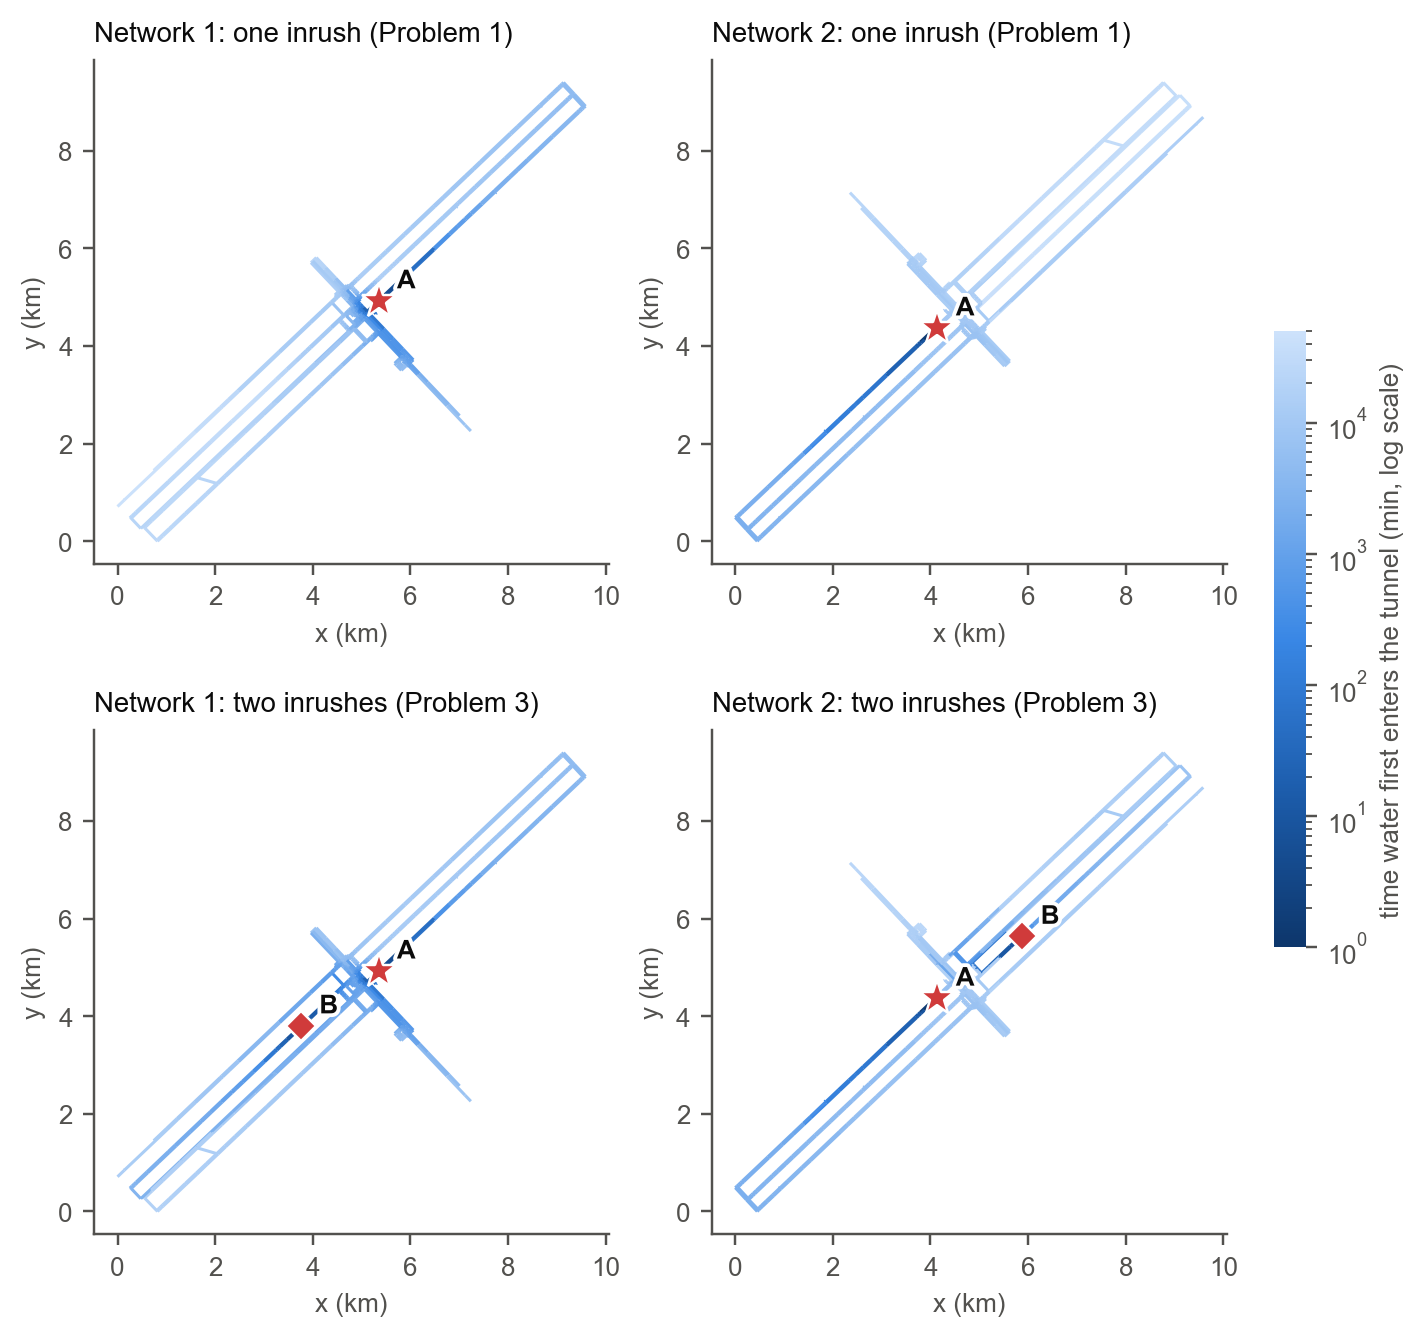
\includegraphics[width=0.92\textwidth]{figures/arrival_maps.png}
  \caption{Time at which water first enters each tunnel, for one inrush point (top) and with the second inrush (bottom).}
  \label{fig:arrival}
\end{figure}

\begin{table}[htbp]
  \centering\small
  \begin{tabular}{@{}l l c c c@{}}
    \toprule
    Network & Case & Median arrival at a junction & Last junction reached & Network full\\
    \midrule
    1 & one inrush (Problem 1)       & 4.4 days & 31.9 days & 34.9 days\\
    1 & two inrushes (Problem 3)     & 1.7 days & 13.8 days & 17.4 days\\
    2 & one inrush (Problem 1)       & 8.2 days & 29.1 days & 34.9 days\\
    2 & two inrushes (Problem 3)     & 5.0 days & 17.1 days & 17.4 days\\
    \midrule
    1 & competition algorithm        & 445 days & $\approx$16{,}000 years & ---\\
    2 & competition algorithm        & \multicolumn{3}{c}{only 28 of 663 junctions ever reached}\\
    \bottomrule
  \end{tabular}
  \caption{Flood timescales. All 663 junctions and 977 tunnels are reached and filled in every new run.}
  \label{tab:flood}
\end{table}

\subsection{Escape routes (Problem 2)}

\begin{table}[htbp]
  \centering\small
  \begin{tabular}{@{}c c c c c c c@{}}
    \toprule
    Network & Miner & Exit & Escape time & Route & Latest start & Dry-mine shortest route\\
            &       &      & (min)       & (km)  & on this route & through the flood (min)\\
    \midrule
    1 & M1 & E1 & 15.9 & 3.57 & 26.6 min & 19.3\\
    1 & M2 & E1 & 12.2 & 2.68 & 7.8 h    & same route\\
    1 & M3 & E1 & 18.1 & 4.10 & 26.8 h   & same route\\
    2 & M1 & E1 & 12.2 & 2.69 & 7.0 days & same route\\
    2 & M2 & E1 & 18.1 & 4.11 & 8.6 days & same route\\
    2 & M3 & E1 & 19.2 & 3.44 & 21.5 h   & 19.7\\
    \bottomrule
  \end{tabular}
  \caption{Fastest escape routes, alert after 1 minute; times from the inrush. ``Latest start'': the latest moment from which the same route still reaches the exit (Corollary~1).}
  \label{tab:p2}
\end{table}

All six miners leave by exit E1 within 12--20 minutes (Table~\ref{tab:p2}, Figure~\ref{fig:p2}). Five of the routes never touch water: the miner walks at 4\,m/s the whole way. For four miners the fastest route is simply the shortest route in a dry mine, because the water never reaches it in time. Two miners are different:
\begin{itemize}[leftmargin=1.5em, itemsep=2pt, topsep=2pt]
  \item \textbf{Network~1, M1} starts near the inrush. The shortest route passes through tunnels that are already wet and would take 19.3 minutes; the fastest route is 40\,m longer but stays dry and takes 15.9. Its latest safe start is 26.6 minutes after the inrush, the tightest margin in Problem~2.
  \item \textbf{Network~2, M3} starts 0.36\,km from the inrush, downhill of it, and cannot avoid wading for part of the way; the best route still saves half a minute over the shortest one.
\end{itemize}

\begin{figure}[htbp]
  \centering
  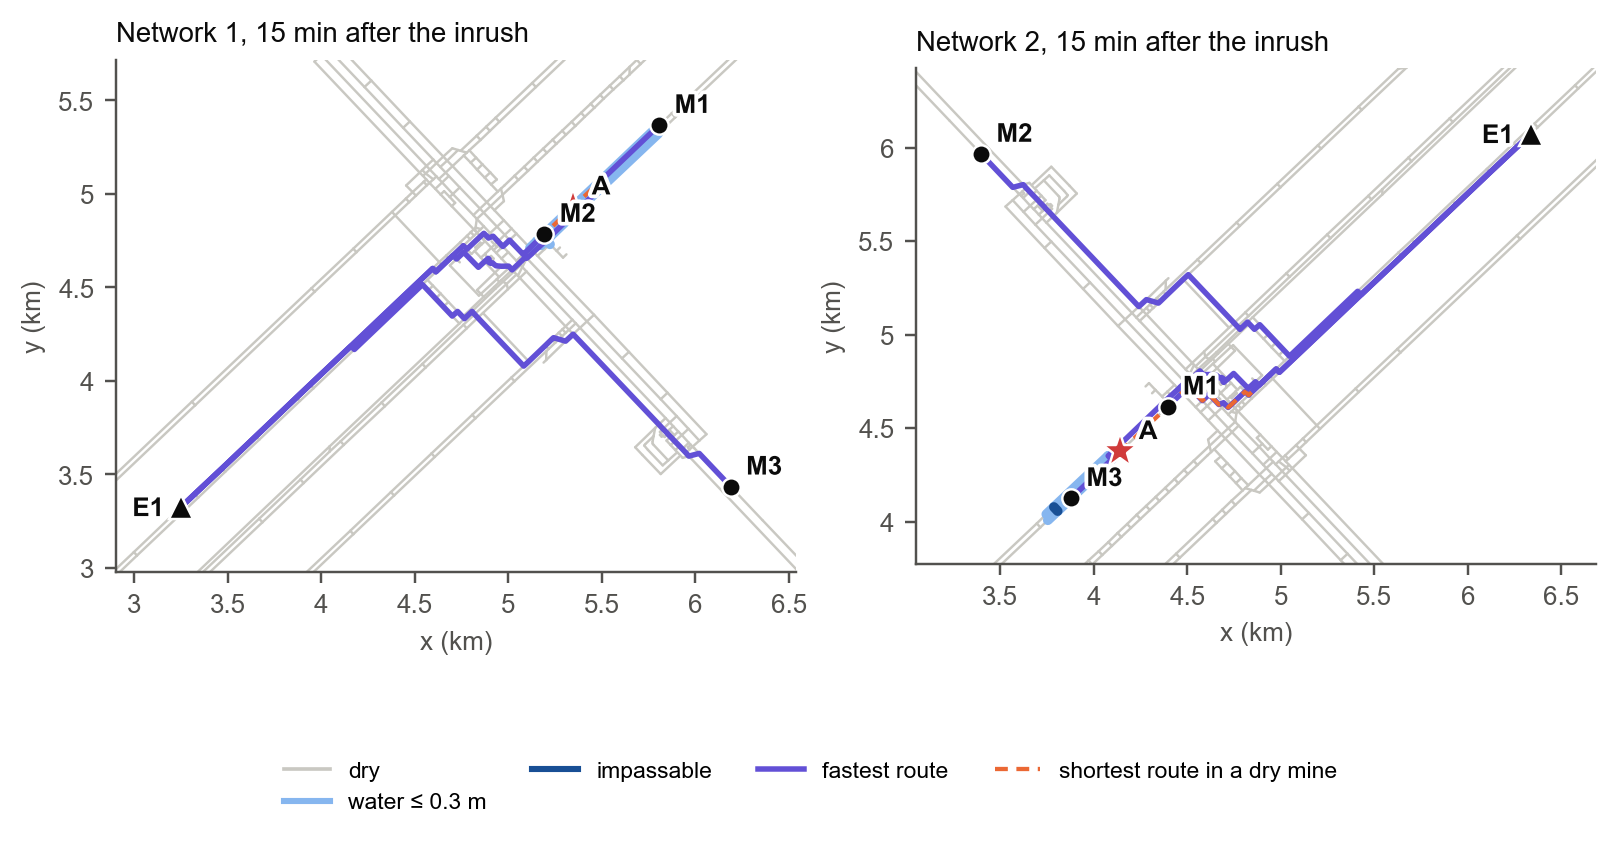
\includegraphics[width=\textwidth]{figures/routes_problem2.png}
  \caption{Fastest routes (Problem~2), with the water 15 minutes after the inrush; enlarged to the area the routes cover.}
  \label{fig:p2}
\end{figure}

\subsection{A second inrush (Problems 3 and 4)}

The second inrush starts 4 minutes (Network~1) or 5 minutes (Network~2) after the first, and the adjusted plan is issued one minute later. At that moment every miner is still inside the mine, part-way along a tunnel. Table~\ref{tab:p4} compares re-planning with keeping the old route.

\begin{table}[htbp]
  \centering\small
  \begin{tabular}{@{}c c c c c c@{}}
    \toprule
    Network & Miner & New exit & \multicolumn{2}{c}{Escape time (min)} & Latest start\\
    \cmidrule(lr){4-5}
            &       &          & re-planned & keep old route & (new route)\\
    \midrule
    1, re-plan at 5 min & M1 & E2 & 16.5 & 20.7 & 95 min\\
      & M2 & E1 & 15.2 & 17.0 & 24.2 min\\
      & M3 & E2 & 18.5 & 26.1 & 56 h\\
    \midrule
    2, re-plan at 6 min & M1 & E1 & 12.4 & 16.3 & 9.1 min\\
      & M2 & E2 & 18.5 & 26.0 & 80 min\\
      & M3 & E2 & 19.8 & 27.1 & 79 min\\
    \bottomrule
  \end{tabular}
  \caption{Re-planning after the second inrush (Problem~4); times from the first inrush.}
  \label{tab:p4}
\end{table}

\begin{figure}[htbp]
  \centering
  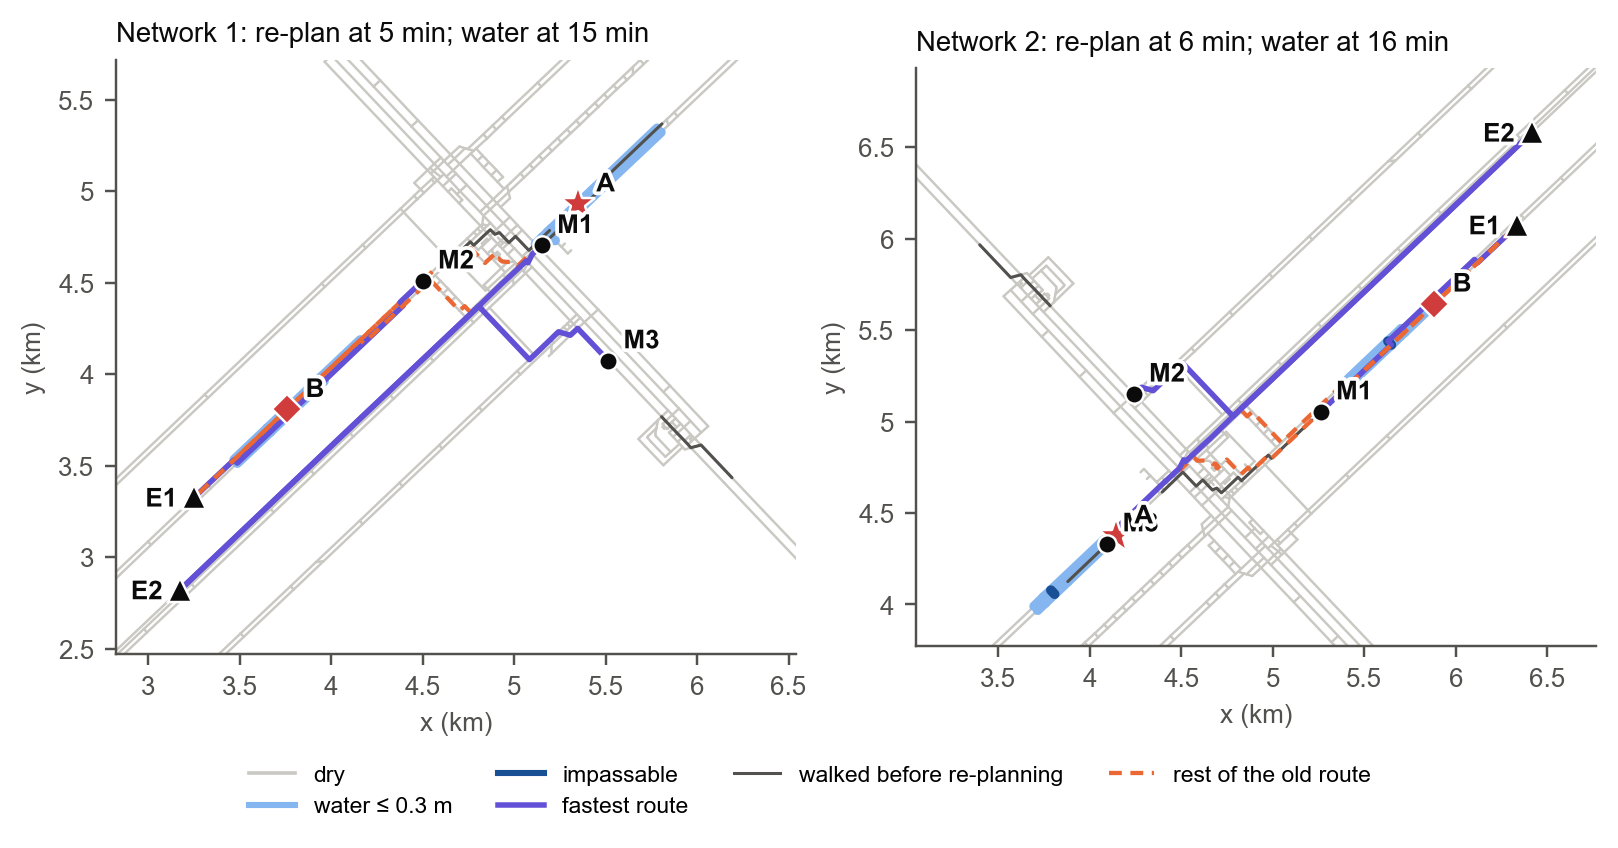
\includegraphics[width=\textwidth]{figures/routes_problem4.png}
  \caption{Re-planned routes (Problem~4). Grey: walked before re-planning; dashed: the rest of the old route; violet: the new route. Water 10 minutes after re-planning.}
  \label{fig:p4}
\end{figure}

All six miners should change route, and four of them change exit (Figure~\ref{fig:p4}): in both networks the second inrush point lies near exit E1 or on the main roadway leading to it. Keeping the old route would not trap anyone, but it would cost up to 7.6 minutes of wading; the second inrush delays the best escape by only 0.2--3.1 minutes compared with Problem~2. The tightest case is Network~2, M1: the new route works only if the miner starts by 9.1 minutes, so an adjusted plan issued about three minutes later than assumed would come too late for that route.

\subsection{Sensitivity}

I changed one parameter at a time and recomputed the floods and all six routes (Table~\ref{tab:sens}). The escape times do not depend on the inflow or on the front depth at all, because the routes that matter stay dry: by Proposition~1 a 10\% larger inrush makes every flood time 9.1\% shorter, but not enough to reach any route in time. Walking speeds in water matter only for the miner who wades. The alert delay matters most. A later alert can force a longer route: for Network~1, M1, the walking time grows by 48\% with an alert after 10 minutes. An immediate alert lets Network~2, M3 leave before the water reaches the first tunnel, and the walk becomes 14\% shorter.

\begin{table}[htbp]
  \centering\small
  \begin{tabular}{@{}l c c c c@{}}
    \toprule
    Parameter & Change & Mean change in walking time & Largest change & Routes that change\\
    \midrule
    Inflow $Q$           & $\pm10\%$ & 0 & 0 & 0\\
    Front depth $h_0$    & $\pm10\%$ & 0 & 0 & 0\\
    Speed with the flow  & $+10\%$ / $-10\%$ & $-0.02\%$ / $+0.02\%$ & 0.14\% & 0\\
    Speed against the flow & $+10\%$ / $-10\%$ & $-0.4\%$ / $+0.5\%$ & 3.0\% & 0\\
    \midrule
    Alert after 0 min    & & $-2.4\%$ & 14\% & 0\\
    Alert after 2 min    & & 0 & 0 & 0\\
    Alert after 5 min    & & $+2.8\%$ & 17\% & 1\\
    Alert after 10 min   & & $+8.4\%$ & 48\% & 1\\
    Alert after 20 min   & & $+8.7\%$ & 48\% & 1\\
    \bottomrule
  \end{tabular}
  \caption{Sensitivity of the six escape routes of Problem~2 (walking time = escape time $-$ alert time; baseline: alert after 1 minute).}
  \label{tab:sens}
\end{table}

\subsection{Checks}
\begin{itemize}[leftmargin=1.5em, itemsep=2pt, topsep=2pt]
  \item \textbf{Conservation} (Proposition~3): after every event, stored volume equals inflow to a relative error below $4\times10^{-15}$, and the last tunnel fills at $V/Q$ to 12 significant digits.
  \item \textbf{Scaling} (Proposition~1): with $1.1\,Q$, all of the roughly 3{,}900 recorded flood times on each network are multiplied by $1/1.1$ to 13 significant digits.
  \item \textbf{Routing}: ten automated tests, including Dijkstra's answer compared with an exhaustive search over all routes on 150 random small networks, and 2{,}000 random checks of Lemma~1 and of the latest-start formula.
  \item \textbf{Resolution}: inserting the exits, miners and second inrush point into the tunnels changes no flood time in Network~1; in Network~2 it changes one region's arrival times by up to 16 hours (on a timescale of weeks) and leaves the median unchanged.
\end{itemize}

% =====================================================================
\section{Worked Example: A Real Mine Plan}\label{sec:example}

To see whether the method works beyond competition data, I applied it to the mining plan of a working longwall coal mine in China \confirm{the provider agrees to its use in anonymized form}. To keep the mine anonymous, all names were removed, the plan was rotated, mirrored and shifted by a random transformation, and elevations are given relative to a hidden reference level.

\subsection{From a CAD drawing to a tunnel graph}
The plan is an AutoCAD drawing with 87 layers. I read it with the open-source LibreDWG library \cite{libredwg} and built the network in four steps:
\begin{enumerate}[leftmargin=2em, itemsep=1pt, topsep=2pt]
  \item \textbf{Tunnels} from the centerline layer (576 lines). Gaps of less than 8\,m between the end of a line and another line --- typically a crosscut ending just short of a roadway --- were bridged (605 gaps); lines were split at every intersection and the largest connected network was kept.
  \item \textbf{Elevation} from the 2{,}347 survey stations labelled with the measured roof elevation; each junction takes the inverse-distance-weighted average of the labels within 300\,m.
  \item \textbf{Width} 5.0\,m, the median distance between the two drawn walls of a roadway. The height is not in the drawing; I kept $H = 3$\,m.
  \item \textbf{Exits}: the four shaft bottoms, joined to the nearest junction (10--66\,m).
\end{enumerate}
The network has 1{,}591 junctions, 2{,}083 tunnels and 248\,km of roadway, with a median gradient of 0.9\%. It is saved in the same format as the competition data, so the same code runs on it unchanged.

\begin{figure}[!htb]
  \centering
  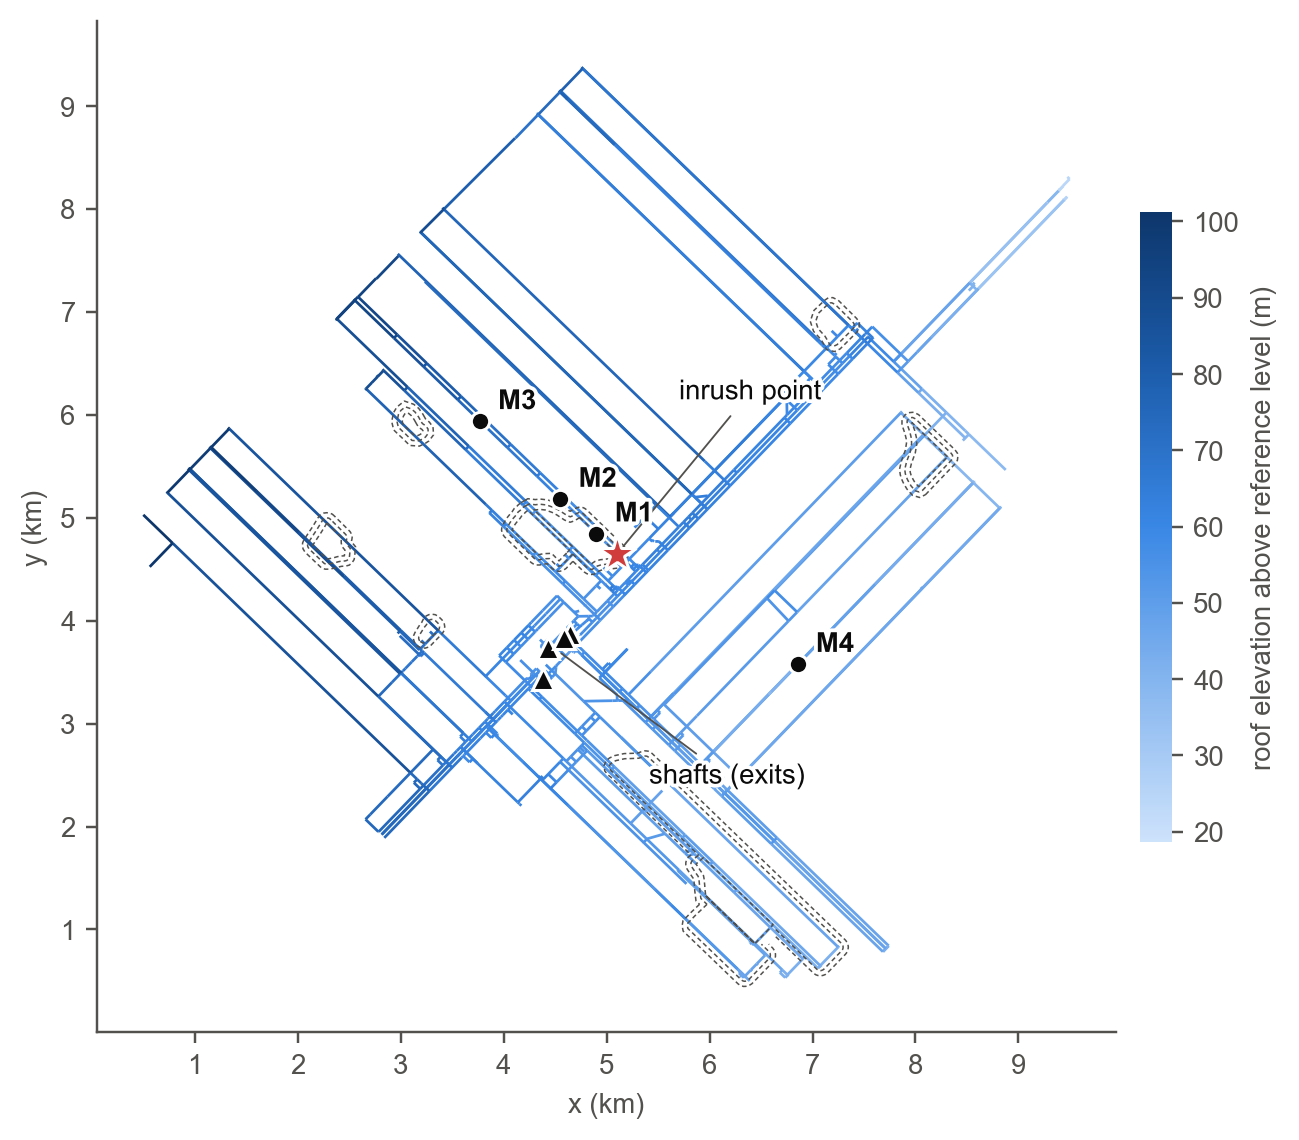
\includegraphics[width=0.72\textwidth]{figures/mine_network.png}
  \caption{Tunnel network extracted from the mine plan (anonymized), coloured by roof elevation, with the water-accumulation zones marked on the plan (dashed), the shafts, the inrush point and four miners.}
  \label{fig:mine}
\end{figure}

\subsection{Scenario}
The plan marks several zones of water accumulated in old workings. I let the zone closest to the shafts break into the roadway that touches it, with $Q = 30\ \mathrm{m^3/min}$ and all other parameters as in the competition. Three miners work at faces 0.3, 0.8 and 1.9\,km (by tunnel) from the inrush whose way out passes near it; a fourth, 4.3\,km away on the other side of the mine, is a control.

\subsection{Results}
The flood stays local for a long time: after one hour 1.7\,km of the 248\,km are wet and 0.5\,km impassable; after a day, 4.4\,km and 3.3\,km. The network fills after 85.9 days, exactly $V/Q$. The competition algorithm on the same network gives a median arrival time of about 300 years.

\begin{table}[htbp]
  \centering\small
  \begin{tabular}{@{}c c c c c@{}}
    \toprule
    Miner & Distance from & Flood-aware route & Dry-mine shortest route & Latest alert that\\
          & the inrush (km) & (min) & through the flood (min) & still leaves a way out\\
    \midrule
    M1 & 0.28 & 7.4  & 10.5 & 4 min 40 s\\
    M2 & 0.77 & 9.4  & 12.6 & 8.2 h\\
    M3 & 1.86 & 14.0 & 23.2 & 2.0 days\\
    M4 & 4.27 & 15.0 & same route & 13 days\\
    \bottomrule
  \end{tabular}
  \caption{Escape on the mine plan, alert after 1 minute; times from the inrush.}
  \label{tab:mine}
\end{table}

\begin{table}[htbp]
  \centering\small
  \begin{tabular}{@{}c cc cc cc@{}}
    \toprule
    Alert after & \multicolumn{2}{c}{M1 (min)} & \multicolumn{2}{c}{M2 (min)} & \multicolumn{2}{c}{M3 (min)}\\
    \cmidrule(lr){2-3}\cmidrule(lr){4-5}\cmidrule(l){6-7}
    (min) & aware & dry-mine & aware & dry-mine & aware & dry-mine\\
    \midrule
    1  & 7.4 & 10.5 & 9.4  & 12.6 & 14.0 & 23.2\\
    3  & 9.4 & 12.5 & 11.4 & 15.5 & 16.0 & 25.2\\
    5  & \multicolumn{2}{c}{no way out} & 13.4 & 22.6 & 18.0 & 27.2\\
    10 & \multicolumn{2}{c}{no way out} & 18.4 & 27.6 & 23.0 & 32.2\\
    \bottomrule
  \end{tabular}
  \caption{Effect of a later alert on the mine plan: flood-aware route vs.\ the shortest route in a dry mine.}
  \label{tab:mine-alert}
\end{table}

\begin{figure}[!htb]
  \centering
  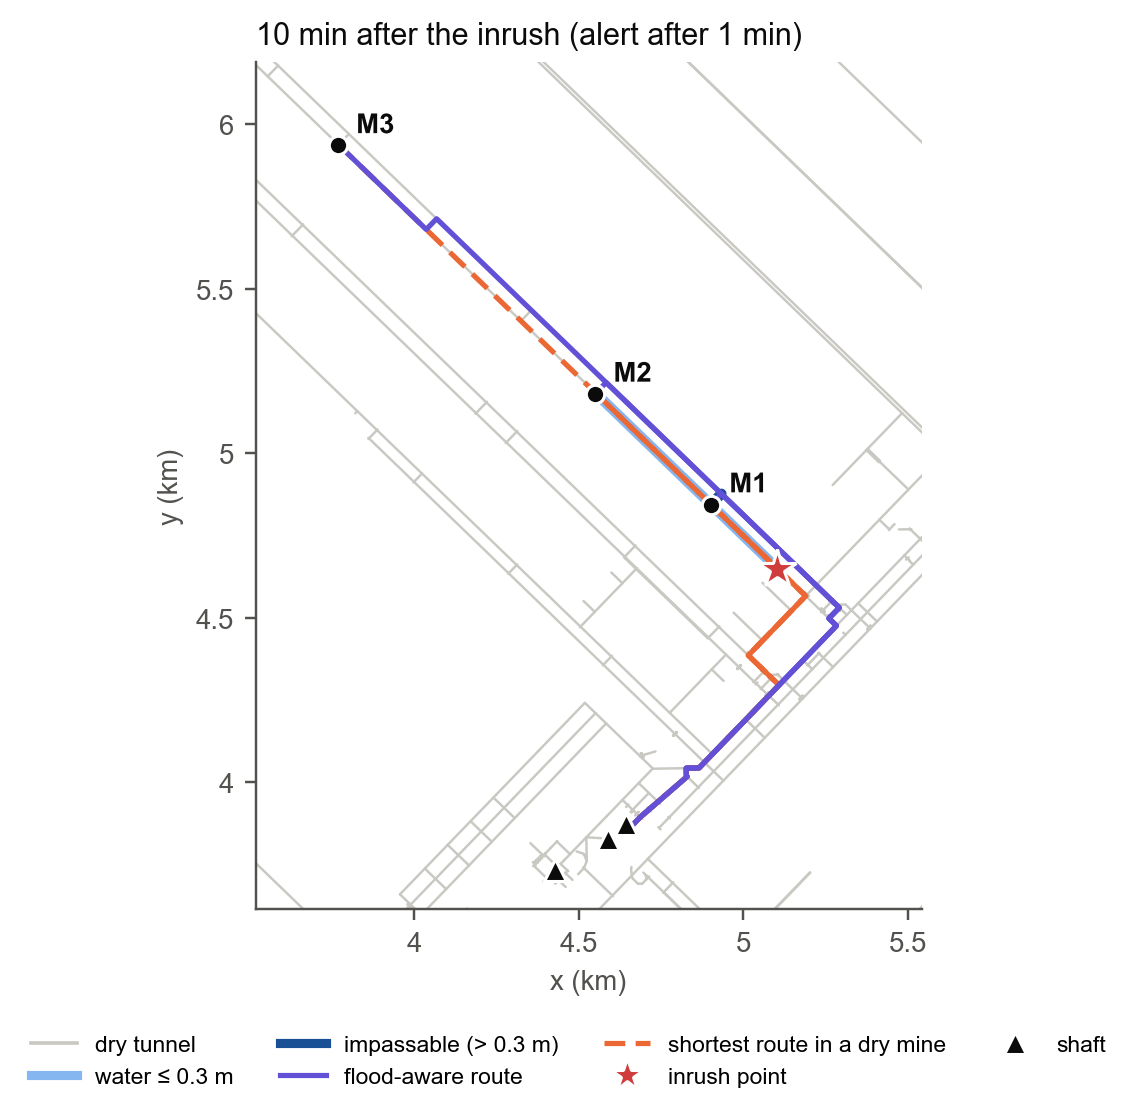
\includegraphics[width=0.6\textwidth]{figures/mine_flood_routes.png}
  \caption{Ten minutes after the inrush: the dry-mine shortest routes (dashed) run along the roadway that the water is filling; the flood-aware routes take the parallel roadway.}
  \label{fig:mine-routes}
\end{figure}

Tables~\ref{tab:mine}--\ref{tab:mine-alert} and Figure~\ref{fig:mine-routes} show three things.
\begin{itemize}[leftmargin=1.5em, itemsep=2pt, topsep=2pt]
  \item \textbf{Knowing where the water is saves minutes.} The dry-mine shortest routes of M1--M3 run along the roadway the water is entering, where they would wade at 1--2\,m/s. The flood-aware routes take the parallel roadway and are 3--9 minutes (up to 40\%) faster.
  \item \textbf{The miner nearest the inrush has minutes, not hours.} M1 works 0.28\,km from the inrush, slightly downhill of it. Unless M1 starts within 4 minutes 40 seconds, no route leads out at all. This latest-alert time, which Corollary~1 makes well defined, is the number a safety officer most needs.
  \item \textbf{Everyone else has time.} M2 and M3 can escape even with an alert hours late, and M4 is unaffected. For this inflow the danger is concentrated within a few hundred metres of the inrush.
\end{itemize}

\paragraph{Checks and limits of the example.} Conservation holds to $4\times10^{-15}$ and the scaling of Proposition~1 holds for all 6{,}251 flood times. The tunnel connections were built automatically and checked by eye against the drawing, not one by one \todo{ask someone who knows the mine to check the network}. Seals and doors marked on the plan are not modelled, elevations are interpolated between survey stations, and the tunnel height is assumed.

% =====================================================================
\section{Limitations}\label{sec:limits}

\begin{itemize}[leftmargin=1.5em, itemsep=2pt, topsep=2pt]
  \item \textbf{Water physics.} The spreading rules are those of the problem statement: a front of fixed depth and an equal split at junctions. Real water is driven by gravity and pressure, and the way water pools (R3--R4) is simplified. A hydraulic model would be more realistic.
  \item \textbf{Uniform depth.} The depth is the same along a whole tunnel; inclined tunnels fill from the bottom in reality.
  \item \textbf{Resolution.} Splitting a tunnel into two can change later flood times slightly (Section~\ref{sec:results}, Checks).
  \item \textbf{Perfect foresight.} The routes assume the whole flood is known in advance. They are the best plan for a correctly predicted flood, not a strategy for a miner who sees only nearby tunnels.
  \item \textbf{No validation.} The results have not been compared with real flooding data or with a physical flow simulation.
  \item \textbf{People.} Fatigue, crowding in narrow tunnels and group decisions are ignored.
\end{itemize}

% =====================================================================
\section{Conclusion}

A flood model for escape planning has to get two things right: where the water goes, and how much of it there is. The competition algorithm got the first roughly right and the second wrong, and its predictions ranged up to thousands of years. With conservation built in, the network fills exactly at $V/Q$, and the model becomes trustworthy over the hours that matter. Because water only rises, escape routing on top of it is first-in, first-out: Dijkstra's algorithm is exact, waiting never helps, and every plan has a well-defined latest safe start. On the competition networks the method solves Problems~1--4 in seconds and shows that after a second inrush every miner should change route. On a real mine plan it shows that a flood-aware route can be 40\% faster, and that the miner nearest the inrush has under five minutes. The natural next steps are a gravity-driven flow model and routing for miners who do not know the future flood.

\paragraph{Code.} \todo{put the code (folders model/, competition/, mine\_example/ without raw/) in a public repository and give the link here; do not attach code listings to the supplement}

\begin{thebibliography}{9}
\setlength{\itemsep}{1pt}\small
\bibitem{cumcm} China Society for Industrial and Applied Mathematics. \emph{China Undergraduate Mathematical Contest in Modeling 2025}, Problem~D: Water-inrush spreading model and escape plans in mines. \confirm{official title and link}
\bibitem{guo} Guo Zhixiong. A brief analysis of mine flooding problems. \emph{Management \& Technology of SME (First Ten-day Issue)}, 2012(8): 156--157. (In Chinese.)
\bibitem{dijkstra} E.~W.~Dijkstra. A note on two problems in connexion with graphs. \emph{Numerische Mathematik}, 1:269--271, 1959.
\bibitem{dreyfus} S.~E.~Dreyfus. An appraisal of some shortest-path algorithms. \emph{Operations Research}, 17(3):395--412, 1969.
\bibitem{orda} A.~Orda and R.~Rom. Shortest-path and minimum-delay algorithms in networks with time-dependent edge-length. \emph{Journal of the ACM}, 37(3):607--625, 1990.
\bibitem{kaufman} D.~E.~Kaufman and R.~L.~Smith. Fastest paths in time-dependent networks for intelligent vehicle-highway systems application. \emph{IVHS Journal}, 1(1):1--11, 1993.
\bibitem{libredwg} GNU LibreDWG, version 0.14. \url{https://www.gnu.org/software/libredwg/}
\end{thebibliography}

% =====================================================================
\newpage
\appendix
\section*{Appendix A. Changes from the Competition Version}
\addcontentsline{toc}{section}{Appendix A}

{\small
\renewcommand{\arraystretch}{1.25}
\begin{tabularx}{\textwidth}{@{}r >{\raggedright\arraybackslash}X >{\raggedright\arraybackslash}p{3.6cm}@{}}
\toprule
& Competition version & Now\\
\midrule
1 & The flood algorithm stored water twice: a covered tunnel filled at its inflow $q$ while passing $q$ on. & Volume-conserving model (Section~\ref{sec:flood}); conservation checked after every event.\\
2 & In Network~2, water never entered an uphill tunnel, so 635 of 663 junctions stayed dry. & Uphill only when no level or downhill tunnel is left (R1, R4); all junctions reached.\\
3 & Flood times of up to ``several years''; the sorted arrival curves were read as ``slow at first, then fast''. & Network full at $V/Q = 35$ days (Proposition~3); spreading slows down (Proposition~2).\\
4 & Sensitivity table: $+10\%$ inflow gave $+3.7\%$ arrival time, and fill time rose for both $\pm10\%$. & Exact $1/\lambda$ scaling (Proposition~1), checked numerically.\\
5 & Walking time from 20 segments, which can misjudge feasibility. & Exact closed form \eqref{eq:exit}.\\
6 & Routing compared the \emph{fraction} filled with 0.3 instead of the \emph{depth}, and used an absolute fill time as a duration. & Impassable when the depth exceeds 0.3\,m ($\tblock$).\\
7 & The code read the data with two header rows, which drops the first junction and tunnel; file names did not match between programs. & One reader for all data; one pipeline.\\
8 & Miners and exits were matched to the nearest junction. & Inserted at their exact positions (Section~2).\\
9 & Depth formula started the rise at 0 instead of $h_0$; route constraint required \emph{every} pair of route nodes to be joined. & Superseded by the new model and Theorem~1.\\
10 & Problems~3--4: method only, no results. & Solved (Tables~\ref{tab:flood} and~\ref{tab:p4}).\\
11 & ``Reverse Dijkstra + A*'' in the text; the code ran a forward search. & Forward time-dependent Dijkstra, proved exact (Theorem~1).\\
\bottomrule
\end{tabularx}
}

\end{document}
